%%% ----------
\section{Панель управления и индикации блока БСП} \label{sec:overview}


%%% ----------
\subsection{Элементы панели управления и индикации}

Внешний вид панели управления и индикации показан на рисунке~\ref{fig:pi}.

\begin{figure}[H]
	\center{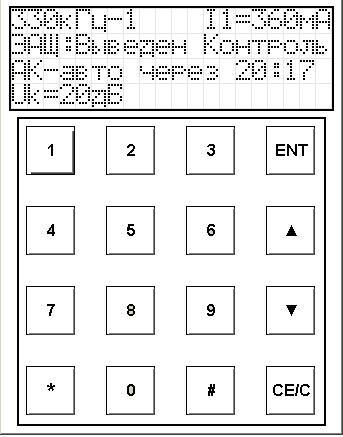
\includegraphics[width=0.4\linewidth]{pi.png}}
	
	\caption{Элементы панели управления и индикации}
	\label{fig:pi}
\end{figure}

Вывод информации в Р400 организован с помощью жидкокристаллического индикатора, имеющего 4 строки по 20 символов. Управление осуществляется посредством 16-кнопочной клавиатуры. Информация на экране обновляется раз в секунду.


%%% ----------
\subsection{Индикация} 


%%% ----------
\subsubsection{Размещение информации в поле индикатора}

Индикатор условно разбит на пять зон, как показано на рисунке~\ref{fig:overview_ind}.

\begin{figure}[H]
	\centering
	
	\begin{tabular}{| M{2.5cm} | M{2.5cm} |}	
		\firsthline
	    0 зона	& 1 зона 				\tabularnewline \hline 
	    \multicolumn{2}{|c|} {2 зона}	\tabularnewline \hline
	    \multicolumn{2}{|c|} {3 зона}	\tabularnewline \hline
	    \multicolumn{2}{|c|} {4 зона}	\tabularnewline 
	    \lasthline 
	\end{tabular} 
	
	\caption{Схемотичное расположение зон на индикаторе} 
	\label{fig:overview_ind}
\end{figure}

Информация, отображаемая в каждой зоне, представлена с сокращениями и, как правило, имеет законченный вид. Далее, по тексту, приводятся пояснения принятых сокращений и месторасположение сообщений по зонам.

Один из вариантов внешнего вида индикатора в исходном (нулевом) уровне показан на рисунке~\ref{fig:overview_level0}. 

\begin{figure}[H]
	\centering
	
	\begin{tabular}{| m{2.5cm}  m{2.5cm} |}
		\firsthline
		330кГц	& \raggedleft I1=360мА 				\tabularnewline 
		\multicolumn{2}{|l|} {ЗАЩ:Введен Контроль}	\tabularnewline 
		\multicolumn{2}{|l|} {АК-авто через 20:17}	\tabularnewline 
		\multicolumn{2}{|l|} {Uk=20дБ}				\tabularnewline
		\lasthline
	\end{tabular} 
	
	\caption{Исходный (нулевой) уровень меню}
	\label{fig:overview_level0}
\end{figure}

0~зона предназначена для вывода информации о текущей дате (Число.Месяц.Год), времени (Часы.Минуты.Секунды) или частоты и номера аппарата (Частота-Номер). Выбор отображаемой информации осуществляется нажатием кнопок \textbf{[4]}~(предыдущий) и \textbf{[6]}~(следующий).

1~зона предназначена для вывода измерений. Листание параметров осуществляется кнопками \textbf{[2]}~(вверх) и \textbf{[8]}~(вниз).

Во второй зоне в нулевом уровне выводятся сообщения, отражающие текущее состояние приемопередатчика сигналов защит (<<ЗАЩ>>), а также сообщения о типе неисправности или предупреждения.

При появлении события, вызывающего предупреждение, информация о текущем состоянии кратковременно, раз в секунду, подменяется соответсвующим сообщением.

В третьей зоне выводится тип автоконтроля и время до следующей проверки канала.

В четвертой зоне всегда показывается уровень контрольной частоты, измеренный при последнем циле проверки канала.

При появлении события, вызывающего сообщение о неисправности (авария), информация о текущем состоянии или предупреждении заменяется аварийной.

Если неисправностей несколько, отображается сообщение старшее по приоритету.


%%% ----------
\subsubsection{Информация о текущем состоянии}

Вид сообщений, отражающих текущее состояние, показан в таблице \ref{tab:overview_reg}.

\begin{tabularx}{\linewidth}{| m{2.5cm} | X | p{11cm} |}
	\caption{Состояния и режимы работы <<ЗАЩ>>}  	\label{tab:overview_reg}	\tabularnewline

	\firsthline
	\centering Поле					& 
	\centering Показания индикатора	& 
	\centering Примечание	
	
	\tabularnewline \hline
	\multirow{ 2}{*}{Режим}	& Введен		&	\tabularnewline \cline{2-3}
							& Выведен		&	\tabularnewline \hline
	\multirow{ 7}{*}{Состояние} & Исходн	& Включение питания, инициализация. \tabularnewline \cline{2-3}
							& Контроль		& Контроль канала, нет сигналов <<Пуск>> и <<Останов>>. \tabularnewline \cline{2-3}		
							& Пуск			& Наличие сигнала <<Пуск>>.\tabularnewline \cline{2-3}			
							& Работа		& Наличие сигнала <<Останов>> при отсутствии сигнала <<Пуск>>. \tabularnewline \cline{2-3}
							& Неиспр		& Восстанавливаемая неисправность. \tabularnewline \cline{2-3}
							& П.неиспр		& Невосстанавливаемая неисправность. \tabularnewline \cline{2-3}
							& Ожидание		& Состояние ожидания для режима <<Выведен>>.\tabularnewline 
	\lasthline								
\end{tabularx}


%%% ----------
\subsubsection{Информация о неисправностях}

При наличии неисправностей в Р400 на экран индикатора выводится информация, показанная на рисунке~\ref{fig:overview_error}.

\begin{figure}[H]
	\centering
	
	\begin{tabular}{| m{2.5cm}  m{2.5cm} |}
		\firsthline
		330кГц	& \raggedleft I1=360мА 				\tabularnewline 
		\multicolumn{2}{|l|} {ЗАЩ:Предупр.l-0001} 	\tabularnewline
		\multicolumn{2}{|l|} {АК-авто через 20:17} 	\tabularnewline 
		\multicolumn{2}{|l|} {Uk=20дБ} 				\tabularnewline 
		\lasthline
	\end{tabular} 
	
	\begin{tabular}{| m{2.5cm}  m{2.5cm} |}
		\firsthline
		 330кГц	& \raggedleft I1=360мА 				\tabularnewline 
		 \multicolumn{2}{|l|} {ЗАЩ:Неиспр. g-0218} 	\tabularnewline 
		 \multicolumn{2}{|l|} {АК-авто через 20:17} \tabularnewline 
		 \multicolumn{2}{|l|} {Uk=20дБ} 			\tabularnewline 
		 \lasthline
	\end{tabular} 
	
	\caption{Информация о неисправностях и предупреждениях}
	\label{fig:overview_error}
\end{figure}

В поле режима выводится сообщение <<Предупр>> (для предупредительной сигнализации) или <<Неиспр>> (для сигнализации неисправности). В поле состояния выводится код неисправности с индексом <<g->> (global) или <<l->> (local). Индекс <<g->> означает, что данная неисправность относится к категории <<глобальных>> (например неисправен блок БСП), и дальнейшая работа аппарата невозможна. Индекс <<l->> означает, что данная неисправность относится к категории <<локальных>> (например неисправен клеммник блока БСЗ), и заблокирована работа только конкретного локального узла аппарата.

При наличии предупредительной сигнализации, сообщение о предупреждении будет подменять информацию о текущем состоянии с частотой примерно два раза в секунду. При этом, если предупреждение одно, то будет выведена его текстовая расшифровка, а если несколько - кодовое обозначение (см. Приложение~\ref{app:err}).

При наличии неисправности в приемопередатчике, сообщение о ней будет выведено на месте текущего состояния. На экран поочередно будут выводится код неисправности и расшифровка самой приоритетной, если их несколько (см. Приложение~\ref{app:err}).


%%% ----------
\subsubsection{Измерения}

В зависимости от текущего выбора, в поле измерений отображаются значения измеряемых параметров, показанных в таблице~\ref{tab:overview_meas}. Переход между отображаемыми параметрами осуществляется нажатием кнопок \textbf{[2]} и \textbf{[8]} (листание вверх/вниз).

\begin{tabularx}{\linewidth}{| M{1cm} | M{3cm}| X |}
	\caption{Измеряемые параметры}  	 
	\label{tab:overview_meas}	\tabularnewline
    
    \firsthline
    
    \centering № п/п & 
    \centering Показания индикатора &     
    \centering Измеряемый параметр
    \tabularnewline \hline  
    \endfirsthead
    
    \multicolumn{3}{l}{Продолжение таблицы \ref{tab:overview_meas}} 
    \tabularnewline \hline 
    \centering № п/п & 
    \centering Показания индикатора &     
    \centering Измеряемый параметр
    \tabularnewline \hline 
  	\endhead
    
    \multicolumn{3}{r}{продолжение следует\ldots} 
	\endfoot
	\endlastfoot
    
    1	& I1	& Выходной ток, мА. \tabularnewline \hline
    2	& U		& Выходное напряжение, В. \tabularnewline \hline
    3	& Uз	& Запас по затуханию для сигналов РЗ, дБ. \tabularnewline \hline
    4	& Uк	& Запас по затуханию для сигналов автоконтроля (АК), дБ. \tabularnewline \hline
    5	& Uш	& Уровень сигнала в рабочей полосе 4~кГц (относительно чувстивтельности), дБ. \tabularnewline \hline
    6	& Sд	& Длительность пауз на выходе приемника, эл. градусы. \tabularnewline 
  
    \lasthline
\end{tabularx} 


%%% ----------
\subsubsection{Дата/время/частота}

0~зона предназначена для вывода информации о ткущей дате (Число.Месяц.Год), времени (Часы:Минуты:Секунды) или частоты и номера аппарата (Частота-номер). Переход между отображением информации осуществляется кнопками \textbf{[4]} (предыдущий) и \textbf{[6]} (следующий).


%%% ----------
\subsubsection{Дополнительная информация}

При отсутствии связи с платой БСП, на экран выводится мигающее сообщение \textbf{<<Нет связи с БСП>>}. Если на экран выводится \textbf{<<????>>}, то это означает, что либо приняты данные, выходящие за диапазон допустимых значений, либо данные вообще не были приняты.

В момент подачи питания также появляется надпись \textbf{<<Инициализация>>}. В это время происходит настройка меню в соответствии с настройками приемопередатчика. Если эта надпись не исчезает с экрана, значит отсутствует связь панели с блоком БСП.
 
 
 %%% ----------
\subsection{Клавиатура} \label{ssec:keyboard}


%%% ----------
\subsubsection{Нулевой уровень меню}

Назначение кнопок на данном уровне меню показано ниже.

\begin{center}
	\begin{tabular}{p{2cm} p{15cm}}
	    \textbf{[2]}, \textbf{[8]} & - листание измеряемого параметра; \tabularnewline
	    \textbf{[4]}, \textbf{[6]} & - листание дата/время/частота; \tabularnewline
	    \textbf{[*]} & - переход на уровень~1 меню. 				
	\end{tabular} 
\end{center}


%%% ----------
\subsubsection{Ввод данных} \label{sssec:keyboard_enter}

При вводе числа с клавиатуры в основном используются кнопки от~1 до~9. Позицию вводимого символа обозначает мигающий курсор. Как только максимально возможное значение симоволов оказывается достигнуто, курсор пропадает. Если не происходит никакой реакции на нажатие кнопки, это означает выход за диапазон допустимых значений (например, попытка ввода 13~месяца).

Завершение ввода подтверждается кнопкой \textbf{[ENT]} (в случае ввода пароля обязательно должно быть 4 введеных символа).

Отмена ввода происходит нажатием на клавишу \textbf{[CE/C]}, стирание предыдущего симовла - \textbf{[$\downarrow$]}. В некоторых случаях возможен переход от одного символа к другому посредством кнопок \textbf{[$\uparrow$]} и \textbf{[$\downarrow$]}.

Некоторые параметры можно изменить только путем выбора соответствующего значения из списка (например, тип защиты). Выбор производится кнопками \textbf{[$\uparrow$]} и \textbf{[$\downarrow$]}. Подтверждение выбора производится нажатием кнопки \textbf{[ENT]}, отмена ввода - \textbf{[CE/C]}.